 %
% File acl2018.tex
%
%% Based on the style files for ACL-2017, with some changes, which were, in turn,
%% Based on the style files for ACL-2015, with some improvements
%%  taken from the NAACL-2016 style
%% Based on the style files for ACL-2014, which were, in turn,
%% based on ACL-2013, ACL-2012, ACL-2011, ACL-2010, ACL-IJCNLP-2009,
%% EACL-2009, IJCNLP-2008...
%% Based on the style files for EACL 2006 by 
%%e.agirre@ehu.es or Sergi.Balari@uab.es
%% and that of ACL 08 by Joakim Nivre and Noah Smith

\documentclass[11pt,a4paper]{article}
\usepackage[hyperref]{acl2018}
\usepackage{times}
\usepackage{latexsym}
\usepackage{amsmath}
\usepackage{tikz}

\setcitestyle{square}
\setcitestyle{numbers}

\usepackage{url}

\aclfinalcopy % Uncomment this line for the final submission
%\def\aclpaperid{***} %  Enter the acl Paper ID here

%\setlength\titlebox{5cm}
% You can expand the titlebox if you need extra space
% to show all the authors. Please do not make the titlebox
% smaller than 5cm (the original size); we will check this
% in the camera-ready version and ask you to change it back.

\newcommand\BibTeX{B{\sc ib}\TeX}
\newcommand{\norm}[1]{\left\lVert#1\right\rVert}

\title{Automatic Tagging of Word Relationships Using Word Embedding}

\author{Roman Tziprun \\
  {\tt romantzr@gmail.com} \\\And
  Eli Shalom \\
  {\tt eli.shalom@gmail.com} \\}

\date{31/8/2018}

\begin{document}
\maketitle
\begin{abstract}
  A great challenge to knowledge construction, manual or automatic, is context understanding. Context can be either the domain or type of entities, of the relationship between entities. For example, "France" and "Paris" are entities of type "Country" and "City" respectively,  and they form a relationship of "Capital". By understanding that the two form a specific relationship, we can improve the efficiency of knowledge construction such as in ontology building, and also improve the performance of semantic-based tasks. In this project we propose an approach for providing textual hints to the context that two entities share.
\end{abstract}
\section{Introduction}
\subsection{Motivation}
Formal knowledge representation is becoming very useful to many semantic tasks in the domain of AI in general and of NLP in particular. For example, clustering of similar web-pages is a very popular feature among search-engines (such as Google-news), and clustering of similar products is very popular in e-commerce sites (such as Amazon-shopping). Additionally, direct semantics understanding tasks which are ontology-based earn a lot from the richness of the ontology on which they are based. This may come into effect with the broadness of entities represented by the ontology (higher recall), or by increased the granularity of entities (higher precision), or by wider relationships representation (improved accuracy).\\
Constructing knowledge is an expensive task. Manual construction requires ontologists to process and formalize information. In Cyc for example, hundreds of person-years were invested and the estimation is that 2000 person years are required to completion. Automatic construction, at the moment, is limited in capabilities and  the successful methods yield mostly entity types and common instances of relations.
\subsection{Goal}
Our project's goal is to reduce the effort required to discover and represent relations between entities in an ontology. We assume that a process for construction already exists and that it requires research from the ontologist. For example, in a geography ontology the entities "France" and "Paris" are expected to appear. Assume very little prior knowledge (very much in this case), then some research is required to figure out that the two entities form some relation and that this relation is "capital-of".\\
We aim to reduce the effort required to understand the existence and details of such relations.
\subsection{High-level approach}
We rely on following assumptions:
\begin{enumerate}
\item It is easier to understand using analogies
\item Analogies can be extracted through Word2vec model
\item A wide and search-able corpus is available
\end{enumerate}
The project aims to provide an understandable context through generalization. The generalization is based on two phases. Firstly, the system receives a pair of terms and using Word2vec extracts pairs that are likely to be analogical to the original pair. A fuzzy comparison on diff vector is used to determine which pairs may form an analogy. Secondly, it searches the corpus for all the documents contains the pairs. The matching documents form a unique vocabulary from which a "pattern" arise. The "pattern" starts from a set of common terms that appear in most documents. The terms are ranked using several heuristics so the most descriptive ones appear on top.
\section{System overview}
The system we developed consists of two parts. The first component (henceforth, referred to as the pairs finder) receives the input which is two words (henceforth, referred to as the source $s$ and the target $t$) and creates a list of word pairs having a similar relation as the relation between $t$ and $s$ by constructing a bipartite graph $G$ in the following manner: 
A word embedding is used to find similar\_sources, a list of 20 words that are most similar to $s$. Let $vec(w)$ be the embedding of the word $w$ in the vector space. For each word $w$ in similar\_sources, we look for 20 words that has a similar relation to $w$ as the relation between $t$ and $s$, this will be the list similar\_targets. This is done by calculating $v = vec(w) + vec(t) - vec(s)$ and looking for the 20 closest words to v. then, from similar\_targets, the word w' which is closest to w is taken, and the edge $e=(w, w')$ is added to $G$ with $weight(e)$ being the cosine distance between them. Then, vertices with degree higher than 4 are removed from the graph to reduce ambiguity. Finally, a maximal matching is computed on the graph by removing the heaviest edges iteratively until there is no vertex with degree higher than 1. This matching constitutes the list of terms which is passed to the next component.

The second component (henceforth, referred to as the label producer) receives this list of pairs as an input and produces a list of words which describe the relation between the words in every pair. Let $x$ and $x'$ be a pair of words in the list returned by the pairs finder. The label producer queries a large corpus (English Wikipedia) for the term "$x$ $x'$" and gets a set of 20 most relevant pages for this term. For every page, a list $L$ of words which appear in all sentences that contain both $x$ and $x'$ is produced. Then, a tf-idf metric is calculated on these words where the term frequency of a word $y$ is is the number of occurrences of $y$ in all sentences containing both $x$ and $x'$ across all 20 pages of the given term. In the last step, a product of all tf-idf values of the same words across the result lists $L$ of all pairs is calculated, and the results are ordered by the highest tf-idf product in descending order, which gives the label list.
\section{Highly recommended}
\subsection{Pairs finding}
This is an intermediate step towards labeling. Given \textit{germany} and \textit{berlin}, the module extracts:
\begin{tabular}{ l l }
  austria & vienna \\
  slovakia & bratislava \\
  denmark & copenhagen \\
  netherlands & amsterdam \\
  poland & warsaw \\
  france & paris \\
  russia & moscow \\
  hungary & budapest \\
  britain & london

\end{tabular}

\subsection{Relation labeling}
This is the main step that given analogies generates candidate terms to label the relation. given the list of analogies generated for \textit{germany} and \textit{berlin}, the modules yields:
\begin{enumerate}
\itemsep0em 
\item \textbf{city}
\item \textbf{capital}
\item largest
\item known
\item airport
\item one
\item located
\item centre
\item listen
\item international
\end{enumerate}
As can be seen, the first two terms are the expected ones to describe the intuitive relationship between \textit{germany} and \textit{berlin}. Since the candidates are sorted by importance, this result is satisfying.

\section{Data, methods and Language-specificity}
The system assumes that a word embedding is provided where:
\begin{enumerate}
\item Words preserve distance, meaning that words that are more similar are closer to one another in the vector space (using a metric like cosine similarity) 
than words that are less similar, where similarity can be defined by context and distributional properties. For example if two words can be 
interchangeable in most context they might be considered very similar \cite{mikolov2013linguistic}.
\item Words preserve analogies, meaning that by calculating $v = vec(x) - vec(y) + vec(z)$, we get that the word $w$ for which $vec(w)$ is 
closest to $v$ should preserve the analogy $x:y::v:z$. For example the vector closest to $v = vec("Brother") - vec("Man") + vec("Woman")$ should be 
the embedding of the word "Sister" \cite{mikolov2013linguistic}.
\end{enumerate}

Such a word embedding is produced by an unsupervised learning algorithm (e.g. word2vec, GloVe, fastText) where the training set is some large corpus (e.g. Wikipedia).
The word embedding is used in the pairs finder component. For simplicity, we used an already train word embedding. Specifically the GloVe model trained 
on Wikipedia with an embedding vector space of dimension $n=50$. The label producer component also uses Wikipedia as a large corpus to generate the 
labels from. It is important to note that our system can be extended to any language simply by changing the trained word vector model to a model 
of a different language and also querying a different language Wikipedia instead of the English one, though some morphological analysis such as 
stemming might be required for other languages \cite{cotterell2015morphological}.

\section{Innovation}
Enrichment of relations is a common task and an evolving one. The vast majority of papers on the topic focus on increasing the number of instances of known relations. Therefore, these tasks are classified as "Knowledge Graph Completion" (such in ~\cite{wang2014knowledge}). Additionally, most tasks assume existing structures which can be repeated ~\cite{ferragina2012fast}, or re-instantiated ~\cite{xie2016representation}. These cases are aimed at the phase which comes after initial knowledge-design (e.g. ontology construction), and rely on a "seed".

Our key differentiating points are:
\begin{enumerate}
\item Goal is improving knowledge design
\item Pure reliance on free-text
\item Strict relation analogy extraction
\item Efficient relation description ranking
\end{enumerate}

A lot of the approaches to formal knowledge construction aim at full automation of the process ~\cite{maedche2001ontology}. Due to the complexity of the task, it is bounded to have some trade-offs with the quality of the constructed knowledge. By relying on human curating, it is more likely that we achieve representation of higher quality. This of course is beneficial only in the context were great quality is indeed required (e.g. a medical application) or in domains where the automatic methods fail.

Since the method discussed here rely manual curating a fuzzier result is expected. Therefore, the system can create keyword based descriptions, instead of pre-structured data such as Wikipedia anchors ~\cite{wang2014knowledge}.

The key innovation point is the ability to communicate by keywords, what is the type of relation that two entities form.

\section{Comparison to existing work}

\subsection{Relation analogies extraction}

We will start by admitting that during the writing of this report we have consulted with Dr. Omer Levy about the task and realized the method we chose is rather limited ~\cite{linzen2016issues}. Additionally, the method of extracting relation analogies through word embeddings is inferior to more recent and advanced methods ~\cite{drozd2016word}.

We will start comparison with one of the original approaches appeared in \textit{Linguistic Regularities in Continuous Space Word Representations}~\cite{mikolov2013linguistic}. The method appears in the paper relates to an evaluation of analogies, such as is "car-cars$\approx$apple-apples", where $\approx$ is a predicate indicating if the two relations are analogical. In that case, the input to the system is a triplet, $w_s,w_t,w_q$, and the goal is to find $w_a$. The method in use is $w_a = \arg \max_w \frac{w \left(w_t-w_s\right)}{\norm{w}\norm{w_t-w_s}}$. We also use a similar method, but using a threshold on the similarity to determine that some candidates may introduce noise.

While remaining in the domain of word embeddings, there are methods to improve the accuracy of evaluation. On example is \textit{3COSADD} which appeared in ~\cite{levy2014linguistic}. The advantage of this method is that it takes into consideration the pair direction, which is tends to represent better semantic relations. Yet, in our model we have not determined whether it is required due to the initial candidates generation process we used.

We realize that it is possible to extend the capturing using machine learning techniques ~\cite{drozd2016word}, yet, some of these techniques may have limitations in domains with broad relation types ~\cite{levy2015supervised}.

In order to overcome some of these limitations, we have limited the type of generalization that is represented by the analogies. We require that the initial seed will be based on entities which are "highly-related" to one of the words from the input. For example, when investigating \textit{germany-berlin}, the seed will be of words that are similar to \textit{germany}. This improves the accuracy of the model in capturing semantic/domain-specific relations. Therefore, it is more likely that relations that will arise from the process will yield more intuitive "hints" in the form of keywords. This method both generates and evaluate candidates for pair analogies.

Secondly, since the source and target candidates are generated in two small spheres (euclidean-wise), it is common to have two different sources forming the same relations with a singe target. In most cases, these relations introduce noise. We use a simple greedy method to disambiguate relations, we think it could have been possible to generalize some more robust methods ~\cite{daelemans1999introduction} for this task.

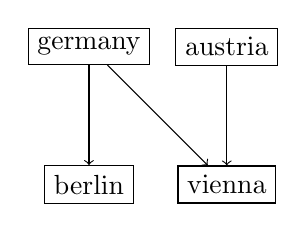
\begin{tikzpicture}[node distance=1.75cm]
  % Dialectics
  \node[draw] (germany) {germany};
  \node[draw, right of=germany] (austria) {austria};
  \node[draw, below of=germany] (berlin) {berlin};
  \node[draw, right of=berlin] (vienna) {vienna};
  
  \draw[->] (germany)  to (berlin);
  \draw[->] (germany) to (vienna);
  \draw[->] (austria) to (vienna);
  
\end{tikzpicture}
\subsection{Description generation}

(Need to explain more on the weights)


\section{Evaluation}

\section{Challenges and what was learned by this project}

Some of the more difficult aspects of our work were parts which involved tuning by trial and error. We tuned a lot of our system's parameters by hand until we received satisfactory results with our evaluation set. The parameters that were tuned include
\begin{enumerate}
\item Similarity threshold: A threshold which is used to filter out words which are not similar enough to the source word when looking for similar sources.
\item Optimal graph degree in the pairs finder. This parameter is used to create a subgraph of the word relations with degree not higher than this value to reduce relational ambiguity.
\item Distance threshold: A threshold which is used to determine if a source is similar enough to the target that was chosen for it. This threshold improved the results by filtering out word pairs which are not very related. We reached the conclusion that we need to incorporate this threshold in our system after we observed that having less pairs but higher accuracy yields better results than having more pairs but lower accuracy.
For example: Providing the pair (australia, canberra) as input to the pairs finder yields the pairs (asian, tokyo), (world, athens), (india, delhi), (britain, ankara), (ireland, dublin), (scotland, christchurch), (england, aberdeen), (united, washington), (canada, ottawa), (uk, overground), (australia, canberra), (zimbabwe, harare), (sydney, melbourne). After introducing the distance threshold, the pairs (asian, tokyo), (united, washington), (uk, overground) and (sydney, melbourne) were eliminated, where 3 out of 4 of these pairs are undesired in this context.

\item The decision of how to combine results in the label producer. The label producer produces a list of labels for every word pair that the pair finder yields. In order to eliminate the less important labels, we used a tf-idf metric for each label, but we've struggled with how to combine the scores of all labels between all pairs. Eventually we reached the conclusion that multiplying these scores gives a good result by trial and error, which makes sense since the product will be higher when the label is more significant (higher tf-idf value) and is repeated across multiple pairs (product over a larger number of elements).
\end{enumerate}


We feel that what hurt our results the most were word ambiguities since a single word has only one embedding even if it has multiple meanings \cite{shi2017jointly}. 
If we had more time, the next thing that we would have done is trained a word embedding of our own on some specific topic like music, science, history, etc. Such a word embedding can be produced on a topical corpus (e.g. Wikipedia articles related to a specific category) and can mitigate issues caused by such ambiguities.


% include your own bib file like this:
%\bibliographystyle{acl}
%\bibliographystyle{numbers}
%\bibliography{acl2018}
\bibliography{acl2018}

\bibliographystyle{acl_natbib}

\appendix

\end{document}
